\documentclass[12pt]{article}

\usepackage{graphicx}
\usepackage{enumerate}
\usepackage{listings}
\usepackage{multicol}



%\linespread{1.6}

\title{Live Map of the DC Bus System: Design}
\author{Ian Will, Jason Cluck}
\date{}

\begin{document}
\maketitle

\begin{abstract}
The Washington Metropolitan Area Transit Authority (WMATA) publishes an API providing access to live bus positions and route details.  There are a few iOS, Android, and Web applications that use this data to help make transit riding more pleasant.  For example, the NextBus application shows the expected arrival time of the next bus for a given route and stop.

However, all current applications are missing some functionality that limit their usefullness.  None of these applications show all bus routes simultaneously on a map.  This limits the transit rider's ability to discover alternate routes.  These current applications also do not take advantage of showing the live bus positions on the map.  A combination of these two points of information would be very helpful for a bus rider.  If the desired bus requires a long wait, a short walk to a nearby station on another route with an approaching bus may provide a better alternative.  This application aims to let the individual riders make informed decisions using all of the available information.

We will use the WMATA developer API to retrieve route details and bus positions from WMATA's servers at regular intervals.  We will then use the Google Maps API to display the route data, updated in real time.  The WMATA developer API places restrictions on frequency of data access--five times per second or 10,000 times per day maximum.  Those limits prohibit accessing the data every time our web page is loaded (were it to be widely used); therefore our application will poll the WMATA servers roughly once every 5 seconds and serve the latest snapshot from our separate web server.  We will use the Ruby on Rails web framework to build a web server that maintains a database of route and position data, updates from WMATA's servers periodically, and displays the data on a map efficiently.  The application will be deployed using the Heroku cloud application platform.
\end{abstract}

\section*{Task Breakdown}
\begin{enumerate}
\item Initial rails setup [Cluck]
\item CSS styling using twitter bootstrap [Cluck]
\item Display map on index page [Cluck]
\item Fetch bus positions from WMATA servers [Will]
\item Store WMATA response in database [Will]
\item Draw markers on map for bus locations [Will]
\item Draw lines on map for bus routes [Will]
\item Show info window when bus marker is clicked, including the following
\begin{enumerate}
\item Route name
\item Schedule deviation (lateness)
\item Time of last position update (data staleness)
\item Headsign
\item Direction
\end{enumerate}
\item Display stops on map
\item Control WMATA polling to avoid exceeding usage limits
\item Display bus stops with markers on map
\item Show info window when stop marker is clicked
	\begin{enumerate}
		\item Show which routes and directions the use the stop
		\item Show next bus wait time projections for each route that uses the stop
	\end{enumerate}
\item Fetch routes from WMATA servers
\item Store routes in database
\item Fetch stops from WMATA servers
\item Store stops in database
\item Layer toggle widget that shows Google traffic overlay, bus markers, and stop markers
\end{enumerate}

\section*{Diagrams}

\begin{figure}[h]
  \caption{System Overview}
  \centering
    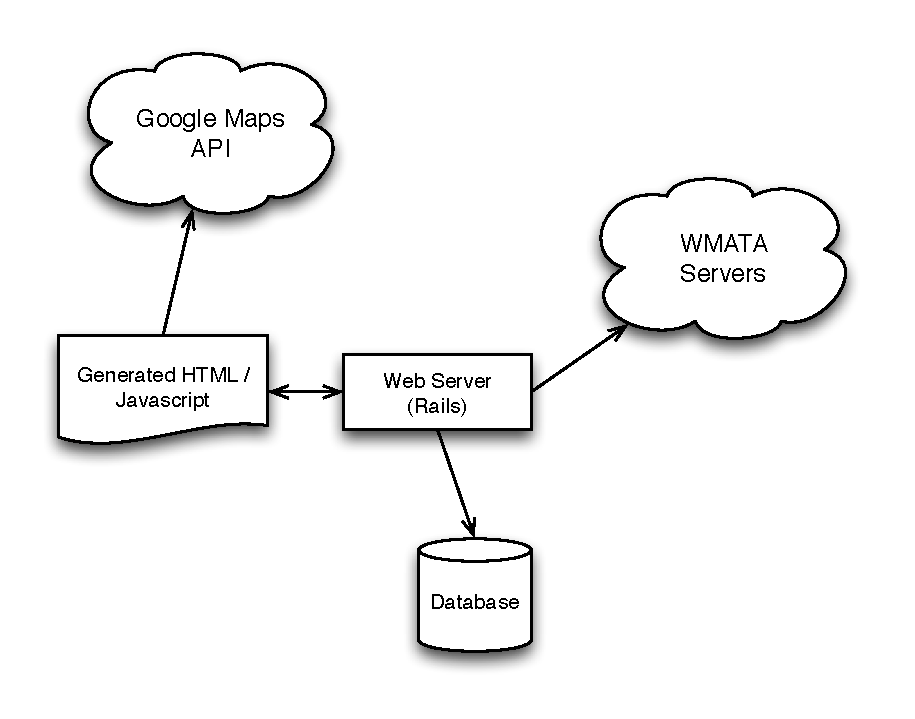
\includegraphics[width=1.0\textwidth]{design.eps}
\end{figure}

\begin{figure}[h]
  \caption{Class Diagram}
  \centering
    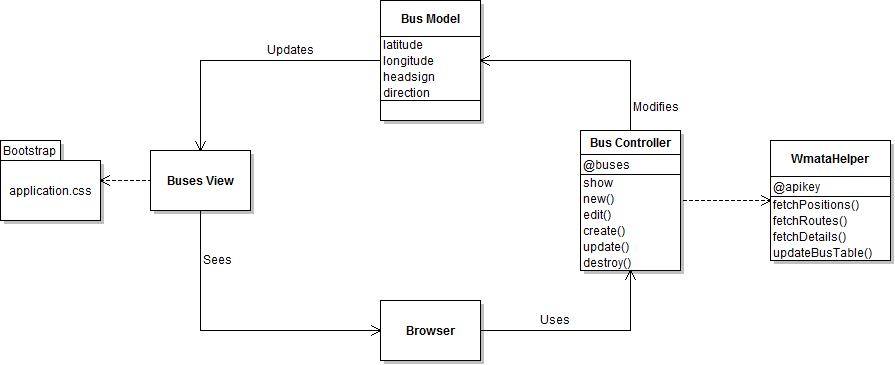
\includegraphics[width=1.0\textwidth]{busTrackerUML.png}
\end{figure}

\begin{figure}[h]
  \caption{Entity Relationship Diagram}
  \centering
    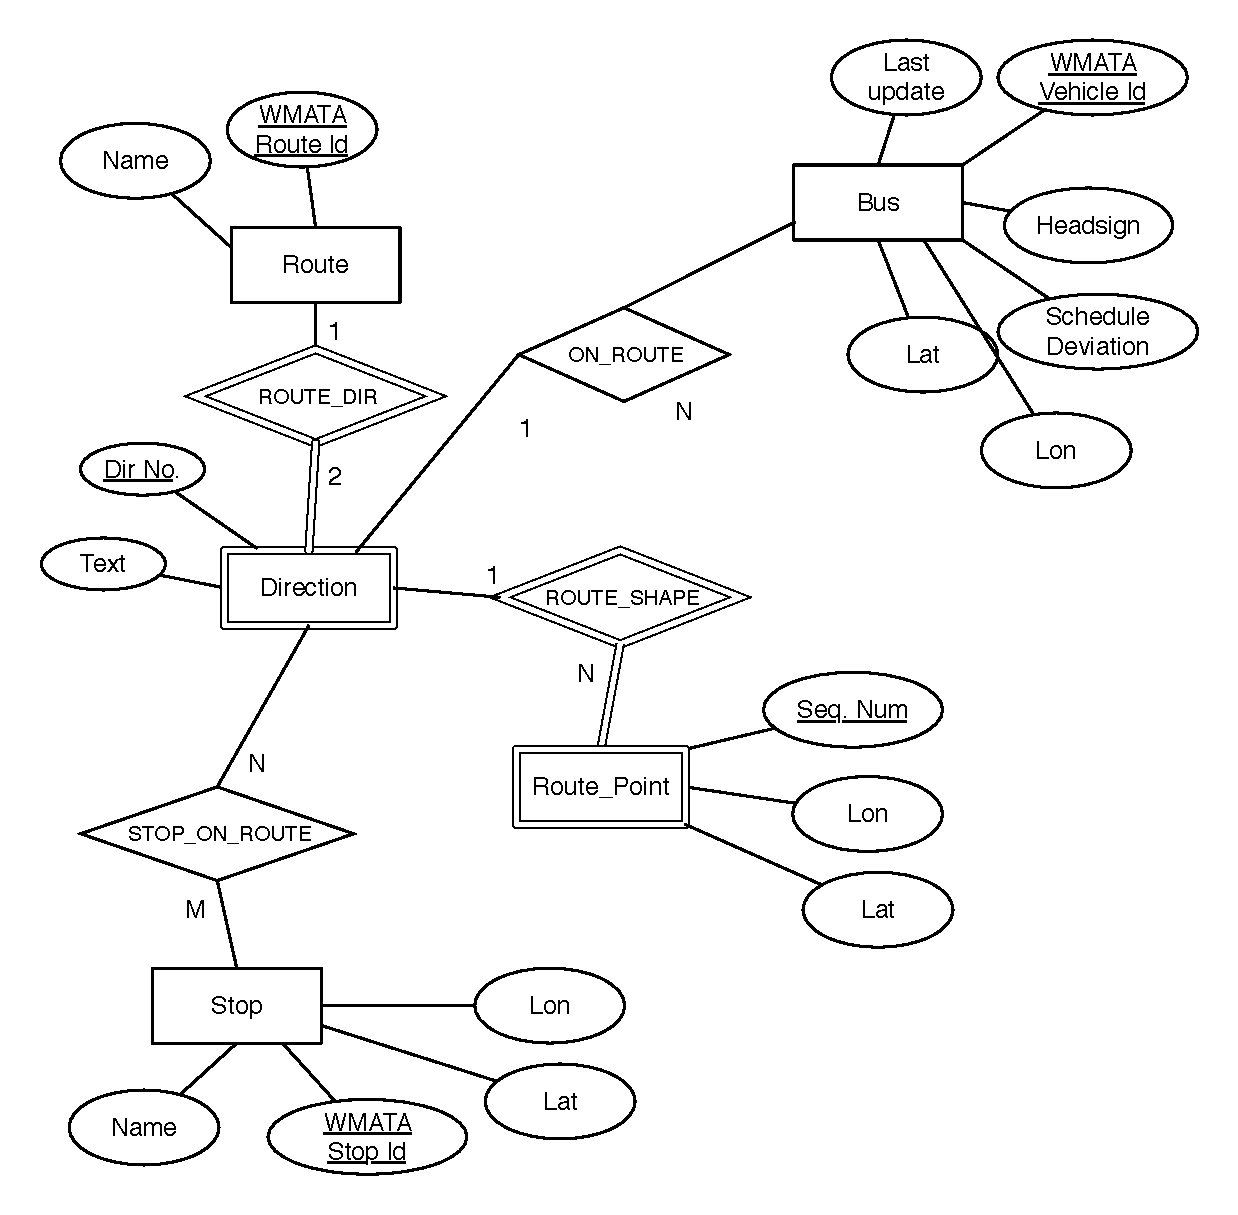
\includegraphics[width=1.0\textwidth]{bus-entity-rel.eps}
\end{figure}


\begin{figure}[h]
  \caption{Database Schema}
  \centering
    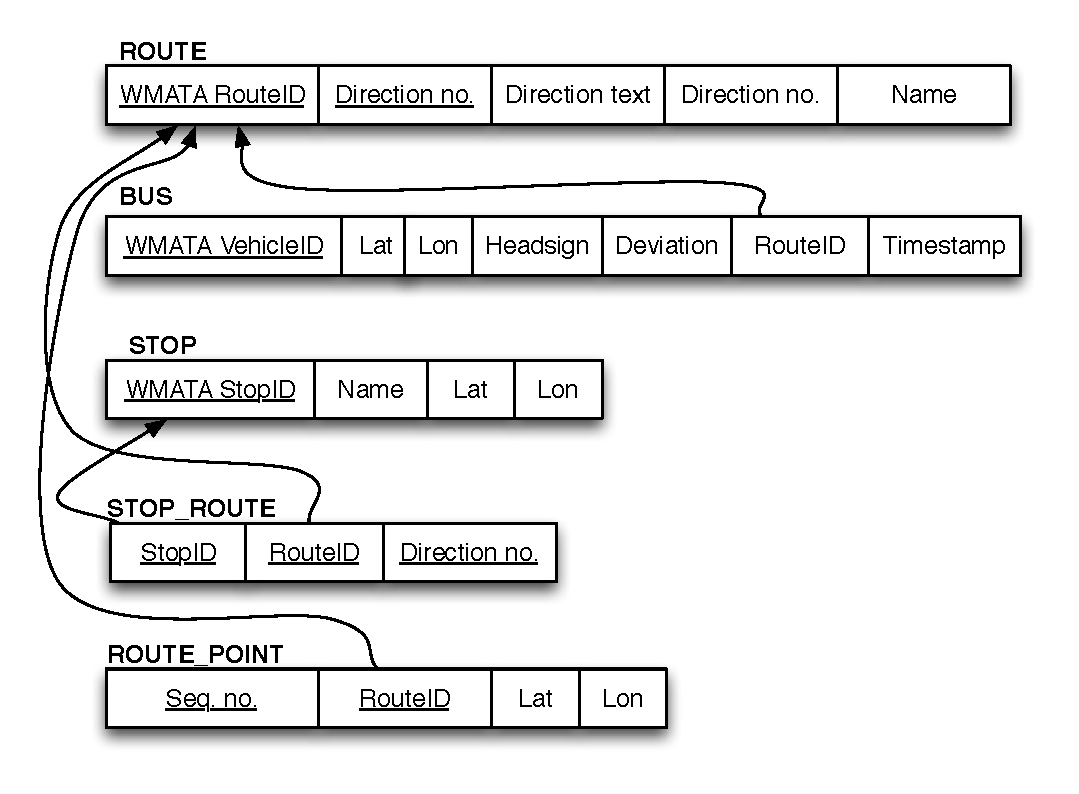
\includegraphics[width=1.0\textwidth]{bus-schema.eps}
\end{figure}


\begin{figure}[h]
  \caption{Sequence Overview}
  \centering
    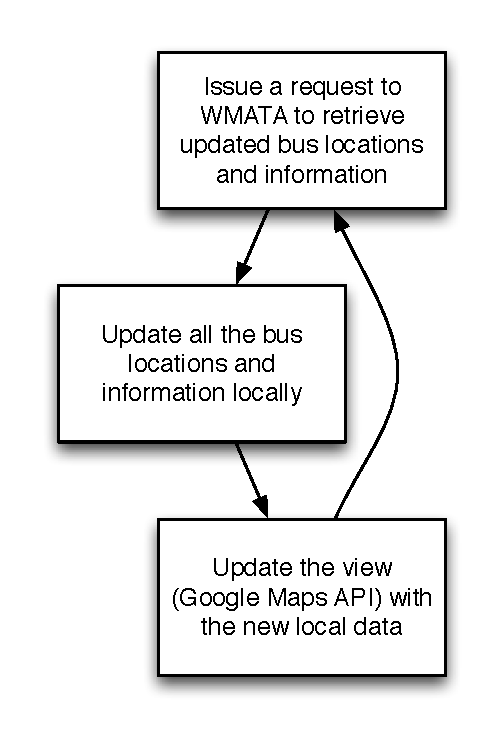
\includegraphics[width=1.0\textwidth]{sequence-diagram.eps}
\end{figure}

\begin{figure}[h]
  \caption{Rails Request Sequence Diagram}
  \centering
    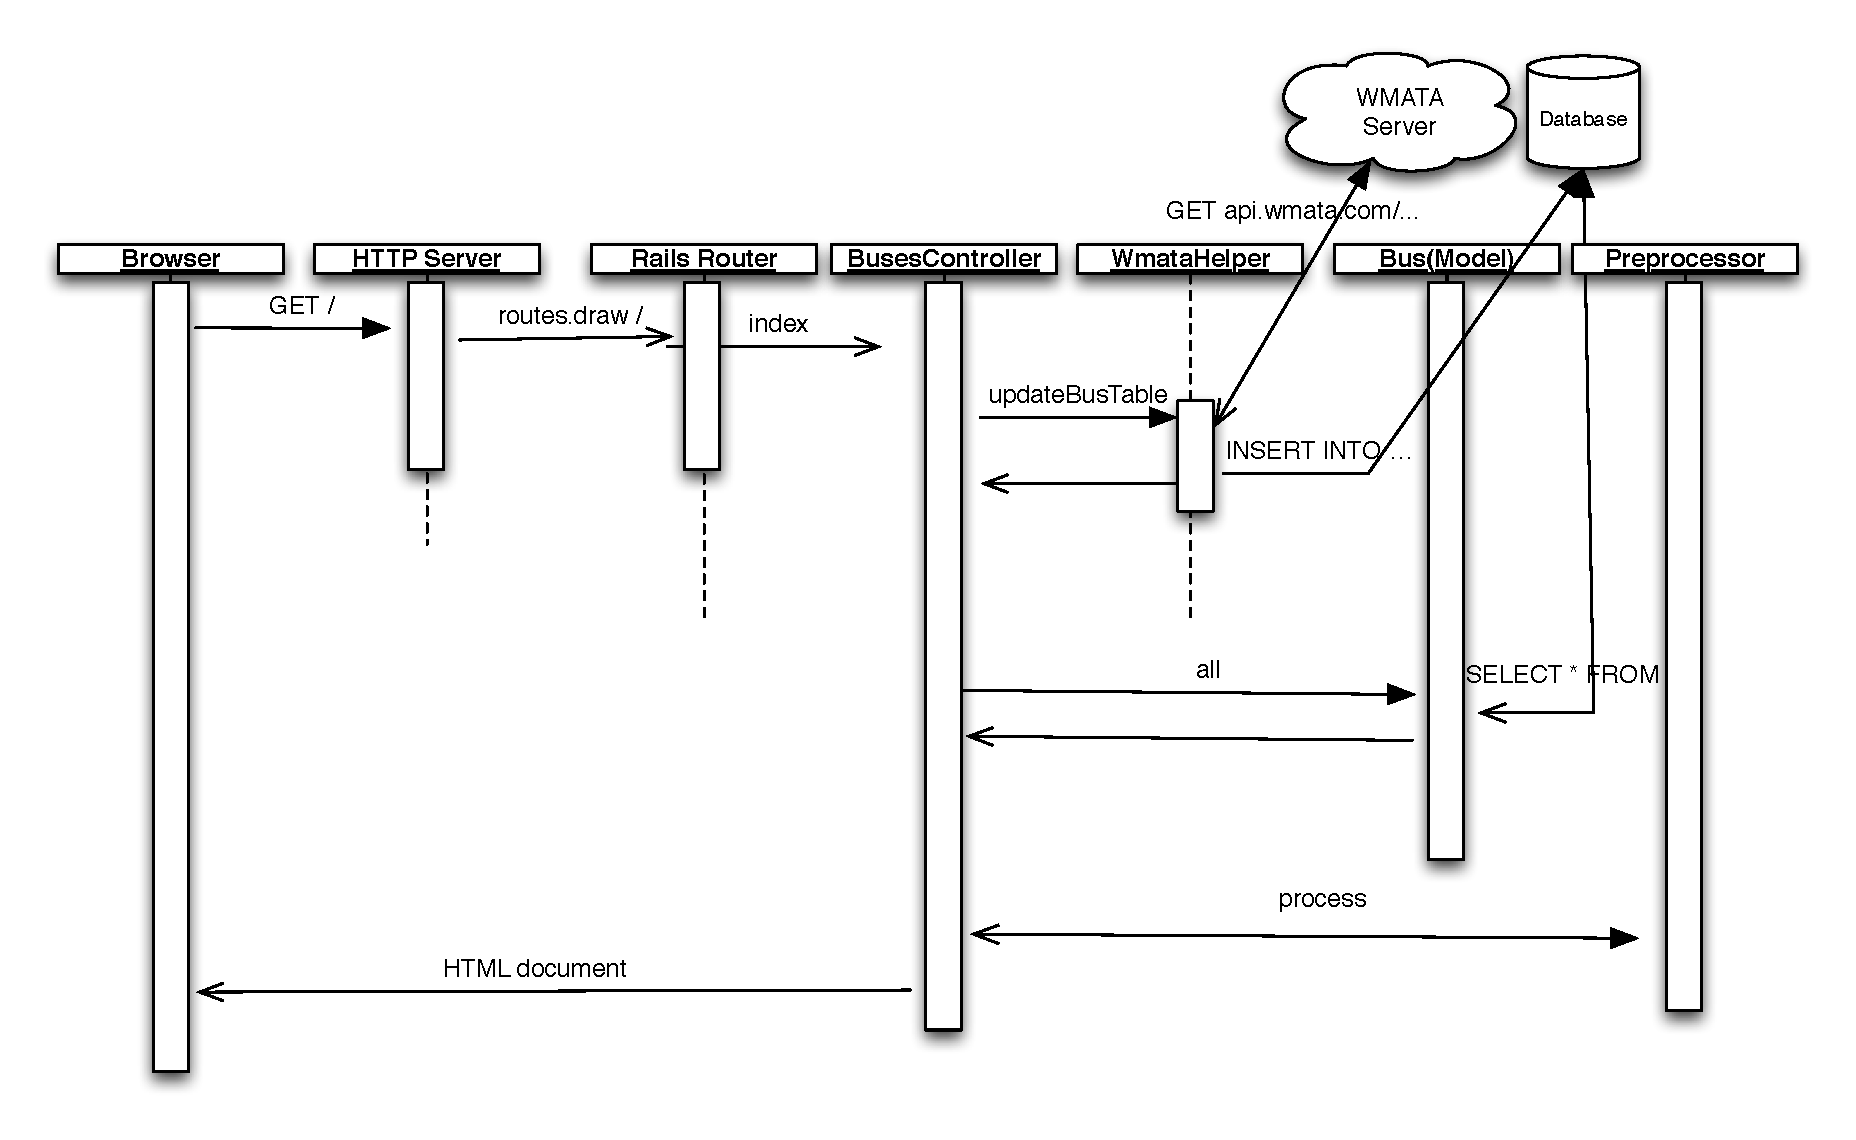
\includegraphics[width=1.0\textwidth]{rails-sequence.eps}
\end{figure}



\end{document}